\section{Battery State of Charge}
Battery state of charge (SOC) also plays a large role in the bus charge problem. As a bus traverses a route, energy is discharged from the battery. If the battery state of charge drops to zero, the bus will power down and become unresponsive. It is therefore important to keep track of bus SOC values while planning charge schedules. 
\par However, because no charge actions are available while on route, SOC values only need be computed while the bus is in the charge station. As these in-station time periods are represented by the charge nodes from figure \ref{fig:busAvailEncode}, SOC variables are in one-one correspondence. Therefore, every charge node$_{i,k}$ has a corresponding SOC value, denoted $d_{i,k}$ as shown in figure \ref{fig:socDiagram}.
\par Charge level progression between $d_{i,k}$ and $d_{i,k+1}$ is influenced by two factors: discharging on route, and charging. The route discharge, denoted $\delta$, represents the energy drawn from the battery in kWh.  When a bus returns from a route, the state of charge is modeled as 
\begin{align}
	d_{i,k+1} = d_{i,k} - \delta_i
\end{align}
where $\delta_i$ is the discharge for Bus $i$'s route as seen in figure \ref{fig:delta}.
\par When a charger connects to a bus, the increase or \textit{gain} in $d$ is denoted $g_{i,k}$, where $i$ and $k$ represent the respective bus and out-going node indices. Figure \ref{fig:dSocDiagram} gives an example where $g_{1,1}$ and $g_{1,2}$ correspond to Bus 1's gain from $t_0$ to $t_1$ and $t_4$ to $t_5$. The gain is used to compute succeeding charge levels as 
\begin{align}\label{eqn:gainInitial}
	d_{i,k+1} = d_{i,k} + g_{i,k}.
\end{align} 

\begin{figure}
	\centering
	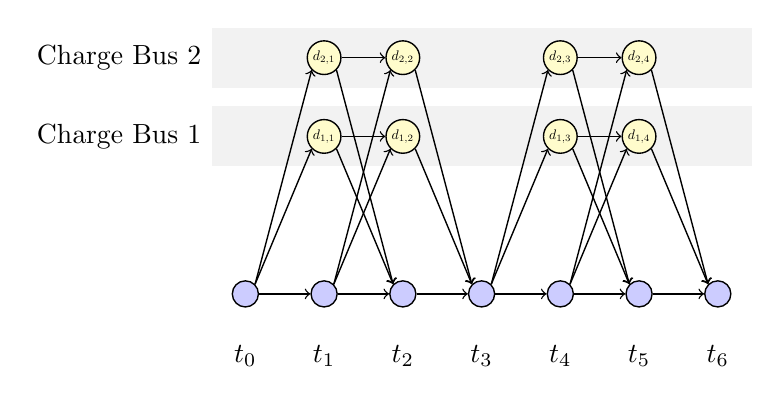
\begin{tikzpicture} 

		\node[rectangle, fill=gray!10, minimum width=2.7in, minimum height=.3in,label=left:Charge Bus 2](bus2Box) at (3,3){};
		\node[rectangle, fill=gray!10, minimum width=2.7in, minimum height=.3in,label=left:Charge Bus 1](bus1Box) at (3,2){};

		\node[circle, fill=blue!20, line width=0.5pt, draw=black, minimum size=0.1in](one) at (0,0){};
		\node[circle, fill=blue!20, line width=0.5pt, draw=black, minimum size=0.1in](two) at (1,0){}; 
		\node[circle, fill=blue!20, line width=0.5pt, draw=black, minimum size=0.1in](three) at (2,0){};
		\node[circle, fill=blue!20, line width=0.5pt, draw=black, minimum size=0.1in](four) at (3,0){};
		\node[circle, fill=blue!20, line width=0.5pt, draw=black, minimum size=0.1in](five) at (4,0){};
		\node[circle, fill=blue!20, line width=0.5pt, draw=black, minimum size=0.1in](six) at (5,0){};
		\node[circle, fill=blue!20, line width=0.5pt, draw=black, minimum size=0.1in](seven) at (6,0){};
		
		\node[circle, fill=yellow!20, line width=0.5pt, draw=black, minimum size=0.1in, inner sep=1pt](eight) at (1,2){\scalebox{0.5}{$d_{1,1}$}};
		\node[circle, fill=yellow!20, line width=0.5pt, draw=black, minimum size=0.1in, inner sep=1pt](nine) at (2,2){\scalebox{0.5}{$d_{1,2}$}};
		\node[circle, fill=yellow!20, line width=0.5pt, draw=black, minimum size=0.1in, inner sep=1pt](ten) at (4,2){\scalebox{0.5}{$d_{1,3}$}}; 
		\node[circle, fill=yellow!20, line width=0.5pt, draw=black, minimum size=0.1in, inner sep=1pt](eleven) at (5,2){\scalebox{0.5}{$d_{1,4}$}}; 

		\node[circle, fill=yellow!20, line width=0.5pt, draw=black, minimum size=0.1in, inner sep=1pt](twelve) at (1,3){\scalebox{0.5}{$d_{2,1}$}};
		\node[circle, fill=yellow!20, line width=0.5pt, draw=black, minimum size=0.1in, inner sep=1pt](thirteen) at (2,3){\scalebox{0.5}{$d_{2,2}$}};
		\node[circle, fill=yellow!20, line width=0.5pt, draw=black, minimum size=0.1in, inner sep=1pt](fourteen) at (4,3){\scalebox{0.5}{$d_{2,3}$}}; 
		\node[circle, fill=yellow!20, line width=0.5pt, draw=black, minimum size=0.1in, inner sep=1pt](fifteen) at (5,3){\scalebox{0.5}{$d_{2,4}$}}; 

		\draw [->, line width=0.5pt] (one.east) -- (two.west);
		\draw [->, line width=0.5pt] (two.east) -- (three.west);
		\draw [->, line width=0.5pt] (three.east) -- (four.west);
		\draw [->, line width=0.5pt] (four.east) -- (five.west);
		\draw [->, line width=0.5pt] (five.east) -- (six.west);
		\draw [->, line width=0.5pt] (six.east) -- (seven.west);

		\draw [->, line width=0.5pt] (one.north east) -- (eight.south west);
		\draw [->, line width=0.5pt] (two.north east) -- (nine.south west);
		\draw [->, line width=0.5pt] (four.north east) -- (ten.south west);
		\draw [->, line width=0.5pt] (five.north east) -- (eleven.south west);
		\draw [->, line width=0.5pt] (eight.south east) -- (three.north west);
		\draw [->, line width=0.5pt] (nine.south east) -- (four.north west);
		\draw [->, line width=0.5pt] (ten.south east) -- (six.north west);
		\draw [->, line width=0.5pt] (eleven.south east) -- (seven.north west);
		\draw [->, line width=0.5pt] (eight.east) -- (nine.west);
		\draw [->, line width=0.5pt] (ten.east) -- (eleven.west); 

		\draw [->, line width=0.5pt] (one.north east) -- (twelve.south west);
		\draw [->, line width=0.5pt] (two.north east) -- (thirteen.south west);
		\draw [->, line width=0.5pt] (four.north east) -- (fourteen.south west);
		\draw [->, line width=0.5pt] (five.north east) -- (fifteen.south west);
		\draw [->, line width=0.5pt] (twelve.south east) -- (three.north west);
		\draw [->, line width=0.5pt] (thirteen.south east) -- (four.north west);
		\draw [->, line width=0.5pt] (fourteen.south east) -- (six.north west);
		\draw [->, line width=0.5pt] (fifteen.south east) -- (seven.north west);
		\draw [->, line width=0.5pt] (twelve.east) -- (thirteen.west);
		\draw [->, line width=0.5pt] (fourteen.east) -- (fifteen.west); 

		\node[rectangle, minimum width=0.3in, minimum height=1.2in,label=below:$t_0$](time0Box) at (0,1){};
		\node[rectangle, minimum width=0.3in, minimum height=1.2in,label=below:$t_1$](time1Box) at (1,1){};
		\node[rectangle, minimum width=0.3in, minimum height=1.2in,label=below:$t_2$](time2Box) at (2,1){};
		\node[rectangle, minimum width=0.3in, minimum height=1.2in,label=below:$t_3$](time3Box) at (3,1){};
		\node[rectangle, minimum width=0.3in, minimum height=1.2in,label=below:$t_4$](time4Box) at (4,1){};
		\node[rectangle, minimum width=0.3in, minimum height=1.2in,label=below:$t_5$](time5Box) at (5,1){};
		\node[rectangle, minimum width=0.3in, minimum height=1.2in,label=below:$t_6$](time6Box) at (6,1){}; 
	\end{tikzpicture}
	\caption{SOC indicators}
	\label{fig:socDiagram}
\end{figure}
\par $g_{i,k}$ is computed using the Constant Current Constant Voltage (CCCV) model as derived in \cite{whitaker_network_2021} which gives:
\begin{align}\label{eqn:CCCV}
	d_{i,k+1} = \bar{a}d_{i,k} - \bar{b}M 
\end{align}
Where $\bar{a}$ is a charge rate dependent constant, $M$ is the battery charge capacity in kWh, and $\bar{b}_l = \bar{a}_l - 1$.
Equations \ref{eqn:gainInitial} and \ref{eqn:CCCV} imply that
\begin{equation}\label{eqn:g}
\begin{aligned}
	& d_{i,k+1} = \bar{a}d_{i,k} - \bar{B}M \\ 
	\Rightarrow & d_{i,k+1} - d_{i,k} = \bar{a}d_{i,k} - \bar{b}M - d_{i,k}\\
	\Rightarrow & g_{i,k}  = \bar{a}d_{i,k} - \bar{b}M - d_{i,k}\\
	\Rightarrow & g_{i,k}  = (\bar{a} - 1)d_{i,k} - \bar{b}M\\
\end{aligned}
\end{equation}
\begin{figure}
	\centering
	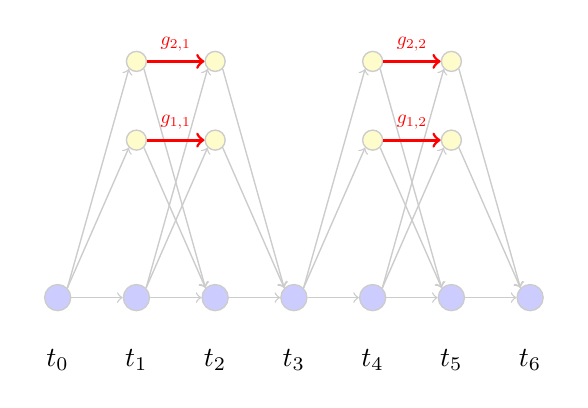
\begin{tikzpicture} 

		\node[circle, fill=blue!20, line width=0.5pt, draw=black!20, minimum size=0.1in](one) at (0,0){};
		\node[circle, fill=blue!20, line width=0.5pt, draw=black!20, minimum size=0.1in](two) at (1,0){}; 
		\node[circle, fill=blue!20, line width=0.5pt, draw=black!20, minimum size=0.1in](three) at (2,0){};
		\node[circle, fill=blue!20, line width=0.5pt, draw=black!20, minimum size=0.1in](four) at (3,0){};
		\node[circle, fill=blue!20, line width=0.5pt, draw=black!20, minimum size=0.1in](five) at (4,0){};
		\node[circle, fill=blue!20, line width=0.5pt, draw=black!20, minimum size=0.1in](six) at (5,0){};
		\node[circle, fill=blue!20, line width=0.5pt, draw=black!20, minimum size=0.1in](seven) at (6,0){};
		
		\node[circle, fill=yellow!20, line width=0.5pt, draw=black!20, minimum size=0.1in, inner sep=1pt](eight) at (1,2){};
		\node[circle, fill=yellow!20, line width=0.5pt, draw=black!20, minimum size=0.1in, inner sep=1pt](nine) at (2,2){};
		\node[circle, fill=yellow!20, line width=0.5pt, draw=black!20, minimum size=0.1in, inner sep=1pt](ten) at (4,2){};
		\node[circle, fill=yellow!20, line width=0.5pt, draw=black!20, minimum size=0.1in, inner sep=1pt](eleven) at (5,2){};

		\node[circle, fill=yellow!20, line width=0.5pt, draw=black!20, minimum size=0.1in, inner sep=1pt](twelve) at (1,3){};
		\node[circle, fill=yellow!20, line width=0.5pt, draw=black!20, minimum size=0.1in, inner sep=1pt](thirteen) at (2,3){};
		\node[circle, fill=yellow!20, line width=0.5pt, draw=black!20, minimum size=0.1in, inner sep=1pt](fourteen) at (4,3){};
		\node[circle, fill=yellow!20, line width=0.5pt, draw=black!20, minimum size=0.1in, inner sep=1pt](fifteen) at (5,3){};

		\draw [->, line width=0.5pt, color=black!20] (one.east) -- (two.west);
		\draw [->, line width=0.5pt, color=black!20] (two.east) -- (three.west);
		\draw [->, line width=0.5pt, color=black!20] (three.east) -- (four.west);
		\draw [->, line width=0.5pt, color=black!20] (four.east) -- (five.west);
		\draw [->, line width=0.5pt, color=black!20] (five.east) -- (six.west);
		\draw [->, line width=0.5pt, color=black!20] (six.east) -- (seven.west);

		\draw [->, line width=0.5pt, color=black!20] (one.north east) -- (eight.south west);
		\draw [->, line width=0.5pt, color=black!20] (two.north east) -- (nine.south west);
		\draw [->, line width=0.5pt, color=black!20] (four.north east) -- (ten.south west);
		\draw [->, line width=0.5pt, color=black!20] (five.north east) -- (eleven.south west);
		\draw [->, line width=0.5pt, color=black!20] (eight.south east) -- (three.north west);
		\draw [->, line width=0.5pt, color=black!20] (nine.south east) -- (four.north west);
		\draw [->, line width=0.5pt, color=black!20] (ten.south east) -- (six.north west);
		\draw [->, line width=0.5pt, color=black!20] (eleven.south east) -- (seven.north west);

		\draw [->, line width=0.5pt, color=black!20] (one.north east) -- (twelve.south west);
		\draw [->, line width=0.5pt, color=black!20] (two.north east) -- (thirteen.south west);
		\draw [->, line width=0.5pt, color=black!20] (four.north east) -- (fourteen.south west);
		\draw [->, line width=0.5pt, color=black!20] (five.north east) -- (fifteen.south west);
		\draw [->, line width=0.5pt, color=black!20] (twelve.south east) -- (three.north west);
		\draw [->, line width=0.5pt, color=black!20] (thirteen.south east) -- (four.north west);
		\draw [->, line width=0.5pt, color=black!20] (fourteen.south east) -- (six.north west);
		\draw [->, line width=0.5pt, color=black!20] (fifteen.south east) -- (seven.north west);
		\draw [->, line width=1pt, color=red] (twelve.east) -- node[above]{\scalebox{0.7}{$g_{2,1}$}}(thirteen.west);
		\draw [->, line width=1pt, color=red] (fourteen.east) -- node[above]{\scalebox{0.7}{$g_{2,2}$}}(fifteen.west); 
		\draw [->, line width=1pt, color=red] (eight.east) -- node[above]{\scalebox{0.7}{$g_{1,1}$}}(nine.west);
		\draw [->, line width=1pt, color=red] (ten.east) -- node[above]{\scalebox{0.7}{$g_{1,2}$}}(eleven.west); 

		\node[rectangle, minimum width=0.3in, minimum height=1.2in,label=below:$t_0$](time0Box) at (0,1){};
		\node[rectangle, minimum width=0.3in, minimum height=1.2in,label=below:$t_1$](time1Box) at (1,1){};
		\node[rectangle, minimum width=0.3in, minimum height=1.2in,label=below:$t_2$](time2Box) at (2,1){};
		\node[rectangle, minimum width=0.3in, minimum height=1.2in,label=below:$t_3$](time3Box) at (3,1){};
		\node[rectangle, minimum width=0.3in, minimum height=1.2in,label=below:$t_4$](time4Box) at (4,1){};
		\node[rectangle, minimum width=0.3in, minimum height=1.2in,label=below:$t_5$](time5Box) at (5,1){};
		\node[rectangle, minimum width=0.3in, minimum height=1.2in,label=below:$t_6$](time6Box) at (6,1){}; 

	\end{tikzpicture}
	\caption{Depiction of which edges increase SOC for the single rate case}
	\label{fig:dSocDiagram}
\end{figure}

\begin{figure}
	\centering
	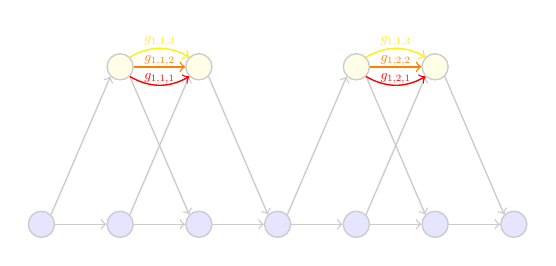
\begin{tikzpicture}[->, line width=0.5pt]
		\node[circle, fill=blue!10, draw=black!20,line width=0.5pt, minimum size=0.1in](one) at (0,0){};
		\node[circle, fill=blue!10, draw=black!20,line width=0.5pt, minimum size=0.1in](two) at (1,0){}; 
		\node[circle, fill=blue!10, draw=black!20,line width=0.5pt, minimum size=0.1in](three) at (2,0){};
		\node[circle, fill=blue!10, draw=black!20,line width=0.5pt, minimum size=0.1in](four) at (3,0){};
		\node[circle, fill=blue!10, draw=black!20,line width=0.5pt, minimum size=0.1in](five) at (4,0){};
		\node[circle, fill=blue!10, draw=black!20,line width=0.5pt, minimum size=0.1in](six) at (5,0){};
		\node[circle, fill=blue!10, draw=black!20,line width=0.5pt, minimum size=0.1in](seven) at (6,0){};
		\node[circle, fill=yellow!10, draw=black!20,line width=0.5pt, minimum size=0.1in](eight) at (1,2){};
		\node[circle, fill=yellow!10, draw=black!20,line width=0.5pt, minimum size=0.1in](nine) at (2,2){};
		\node[circle, fill=yellow!10, draw=black!20,line width=0.5pt, minimum size=0.1in](ten) at (4,2){}; 
		\node[circle, fill=yellow!10, draw=black!20,line width=0.5pt, minimum size=0.1in](eleven) at (5,2){}; 
		\draw [line width=0.5pt,color=black!20] (one.east) -- (two.west);
		\draw [line width=0.5pt,color=black!20] (two.east) -- (three.west);
		\draw [line width=0.5pt,color=black!20] (three.east) -- (four.west);
		\draw [line width=0.5pt,color=black!20] (four.east) -- (five.west);
		\draw [line width=0.5pt,color=black!20] (five.east) -- (six.west);
		\draw [line width=0.5pt,color=black!20] (six.east) -- (seven.west);
		\draw [line width=0.5pt,color=black!20] (one.north east) -- (eight.south west);
		\draw [line width=0.5pt,color=black!20] (two.north east) -- (nine.south west);
		\draw [line width=0.5pt,color=black!20] (four.north east) -- (ten.south west);
		\draw [line width=0.5pt,color=black!20] (five.north east) -- (eleven.south west);
		\draw [line width=0.5pt,color=black!20] (eight.south east) -- (three.north west);
		\draw [line width=0.5pt,color=black!20] (nine.south east) -- (four.north west);
		\draw [line width=0.5pt,color=black!20] (ten.south east) -- (six.north west);
		\draw [line width=0.5pt,color=black!20] (eleven.south east) -- (seven.north west);

		\draw [color=yellow,-,line width=0.5pt] (eight.north east) edge[->,bend left]node[above=-3pt]{\scalebox{0.5}{$g_{1,1,3}$}}(nine.north west);
		\draw [color=orange,line width=0.5pt] (eight.east) -- node[above=-3pt]{\scalebox{0.5}{$g_{1,1,2}$}}(nine.west);
		\draw [color=red,-,line width=0.5pt] (eight.south east) edge[->, bend right]node[above=-3pt]{\scalebox{0.5}{$g_{1,1,1}$}}(nine.south west);

		\draw [color=yellow,-, line width=0.5pt] (ten.north east) edge[->, bend left]node[above=-3pt]{\scalebox{0.5}{$g_{1,1,3}$}}(eleven.north west);
		\draw [color=orange,line width=0.5pt] (ten.east) -- node[above=-3pt]{\scalebox{0.5}{$g_{1,2,2}$}}(eleven.west); 
		\draw [color=red,-, line width=0.5pt] (ten.south east) edge[->, bend right]node[above=-3pt]{\scalebox{0.5}{$g_{1,2,1}$}}(eleven.south west);
	\end{tikzpicture}
	\caption{Multi-Rate Charging}
	\label{fig:multiRateChargeEdges}
\end{figure} 

Equation \ref{eqn:g} holds when a charger is connected to a bus.  This is the case when the edge corresponding to $g_{i,k}$ has a weight of $1$. When the weight equals $0$, then $g_{i,k}$ must also equal zero. These two situations can be described using a switching constraint known as the \textit{big M} technique. This is used to switch between equation \ref{eqn:g}, and $g_{i,k} = 0$ as follows: 
\begin{equation}\label{eqn:bigMIneq}
\begin{aligned}
	& \begin{dcases} 
		\begin{array}{l}
		g_{i,k} = d_{i,k}(\bar{a} - 1) - \bar{b}M
		\end{array} & x_{i,k} = 1\\
		\begin{array}{l}
		g_{i,k} = 0
		\end{array} & x_{i,k} = 0\\
	\end{dcases} \\ 
	\Rightarrow & 
	\begin{dcases} 
		\begin{array}{l}
		g_{i,k} \le d_{i,k}(\bar{a} - 1) - \bar{b}M\\
		g_{i,k} \ge d_{i,k}(\bar{a} - 1) - \bar{b}M\\
		\end{array}
		& x_{i,k} = 1 \\
		\begin{array}{l}
		g_{i,k} \le 0 \\
		g_{i,k} \ge 0 \\
		\end{array} & x_{i,k} = 0\\
    	\end{dcases} 
\end{aligned}
\end{equation}
where $x_{i,k}$ is the weight of the edge corresponding to $g_{i,k}$.  The piecewise function in \ref{eqn:bigMIneq} can be rewritten as 
\begin{equation}\label{eqn:bigM2}
 \begin{aligned} 
	 &\begin{dcases} 
		\begin{array}{l}
		g_{i,k} \le d_{i,k}(\bar{a} - 1) - \bar{b}M\\
		g_{i,k} \ge d_{i,k}(\bar{a} - 1) - \bar{b}M\\
		\end{array}
		& x_{i,k} = 1 \\
		\begin{array}{l}
		g_{i,k} \le 0 \\
		g_{i,k} \ge 0 \\
		\end{array} & x_{i,k} = 0\\ 
	\end{dcases} \\
	\Rightarrow & 
	 \begin{array}{l}
		 g_{i,k} \le d_{i,k}(\bar{a} - 1) - \bar{b}M - M(1 - x_{i,k})\\
		g_{i,k} \ge d_{i,k}(\bar{a} - 1) - \bar{b}M\\
		 g_{i,k} \le 0 + Mx_{i,k} \\
		g_{i,k} \ge 0 \\
	 \end{array}
\end{aligned}
\end{equation}
The results of equation \ref{eqn:bigM2} obtain a switching effect.  When $x_{i,k} = 1$, equation \ref{eqn:bigM2} becomes 
\begin{equation}
	\begin{aligned}
		\color{blue}{g_{i,k}}  &\color{blue}{\le d_{i,k}(\bar{a} - 1) - \bar{b}M} \\
		\color{blue}{g_{i,k}}  &\color{blue}{\ge d_{i,k}(\bar{a} - 1) - \bar{b}M} \\
		\color{red}{g_{i,k}} & \color{red}{\le M} \\
		\color{red}{g_{i,k}} & \color{red}{\ge 0}.  
	\end{aligned}
\end{equation}
Because $g$ can never exceed the charge capacity of the battery, the bottom two constraints are inactive and $g$ is both less than or greater than equation \ref{eqn:g}, making it equal.  When the edge is inactive, or $x_{i,k} = 0$, equation \ref{eqn:bigM2} becomes
\begin{equation}
	\begin{aligned}
		\color{red}{g_{i,k}}  &\color{red}{\le d_{i,k}(\bar{a}_l - 1) - \bar{b}_lM - M} \\
		\color{red}{g_{i,k}}  &\color{red}{\ge d_{i,k}(\bar{a}_l - 1) - \bar{b}_lM} \\
		\color{blue}{g_{i,k}} &\color{blue}{\le 0} \\
		\color{blue}{g_{i,k}} &\color{blue}{\ge 0}.  
	\end{aligned}
\end{equation}
where the top two constraints become inactive and $g$ is both less than and greater than 0, making it equal.

\par Equation \ref{eqn:bigM2} can be expressed in linear form as 
\begin{equation}\label{eqn:chargeConstraints}
	\begin{aligned} 
		-g_{m,k,l} + d_{m,k,l}(\bar{a}_l - 1) + x_{m,k,l} &\le M(\bar{b}_l + 1) \\
		 g_{m,k,l} - d_{m,k,l}(\bar{a}_l - 1)  &\le  - \bar{b}_lM \\
		 g_{m,k,l} - Mx_{m,k,l} &\le 0 \\
		-g_{m,k,l} &\le 0.  
	\end{aligned}
\end{equation}
\par The constraints for state of charge are circumstantially dependent. Each $d_{m,k,l}$ must be defined by a set of constraints which are defined by either initial conditions, previous graphs, route discharge, or $g_{m,k,l}$ variables.
\par Initial conditions and previous graphs are straight forward.  Initial conditions are given as an equality constraint.  For example, if $d_0$ was initialized to 80 kWh, the constraint would be $d_0 = 80$.  To initialize to the value of a previous graph, use an equality constraint.  
\par Suppose we modeled early morning and day-time operations and had two corresponding graphs. The final node of graph one would be equivalent to the first node of graph two in the temporal sense and the corresponding $d_{m,l,k}$ values would also be equated as $d_{\text{Graph 1}} - d_{\text{Graph 2}} = 0$.
\par $d_{m,l,k}$ values corresponding to available charge times are expressed as a sum of $g_{m,k,l}$ values given in equation \ref{eqn:chargeConstraints} such that
\begin{align*}
	d_{m,k + 1} = d_{m,k} + \sum_l{g_{m,k,l}}
\end{align*}
or as given in linear form,
\begin{align}
	d_{m,k+1} - d_{m,k} - \sum_l{g_{m,k,l}} = 0.
\end{align}
\par The final case deals with battery discharge over a route.  As seen in figure \ref{fig:delta}, discharge values, also refered to as $\delta$ represent the power expenditure overa route.  This expenditure is modeled as a withdrawel from the resevour in a battery and was calibrated from data received from the Utah Transit Authority.  In figure \ref{fig:delta}, the SOC constraints corresponding to $\delta_1$ would be as follow:
\begin{align*}
	d_{1,3} = d_{1,2} - \delta_1
\end{align*}
or in linear form,
\begin{align}
	d_{1,2} - d_{1,3} = \delta_1.
\end{align}
\begin{figure}
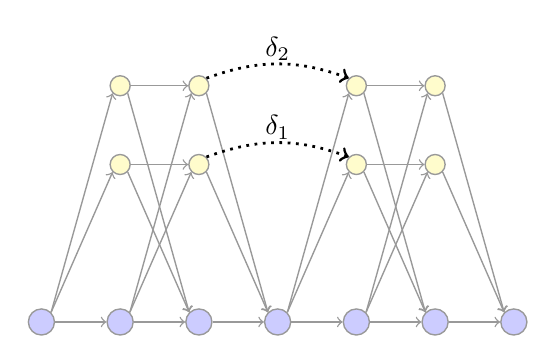
\begin{tikzpicture}
	\node[circle, fill=blue!20, line width=0.5pt, draw=black!40, minimum size=0.1in](one) at (0,0){};
	\node[circle, fill=blue!20, line width=0.5pt, draw=black!40, minimum size=0.1in](two) at (1,0){}; 
	\node[circle, fill=blue!20, line width=0.5pt, draw=black!40, minimum size=0.1in](three) at (2,0){};
	\node[circle, fill=blue!20, line width=0.5pt, draw=black!40, minimum size=0.1in](four) at (3,0){};
	\node[circle, fill=blue!20, line width=0.5pt, draw=black!40, minimum size=0.1in](five) at (4,0){};
	\node[circle, fill=blue!20, line width=0.5pt, draw=black!40, minimum size=0.1in](six) at (5,0){};
	\node[circle, fill=blue!20, line width=0.5pt, draw=black!40, minimum size=0.1in](seven) at (6,0){};
	
	\node[circle, fill=yellow!20, line width=0.5pt, draw=black!40, minimum size=0.1in, inner sep=1pt](eight) at (1,2){};
	\node[circle, fill=yellow!20, line width=0.5pt, draw=black!40, minimum size=0.1in, inner sep=1pt](nine) at (2,2){};
	\node[circle, fill=yellow!20, line width=0.5pt, draw=black!40, minimum size=0.1in, inner sep=1pt](ten) at (4,2){};
	\node[circle, fill=yellow!20, line width=0.5pt, draw=black!40, minimum size=0.1in, inner sep=1pt](eleven) at (5,2){};

	\node[circle, fill=yellow!20, line width=0.5pt, draw=black!40, minimum size=0.1in, inner sep=1pt](twelve) at (1,3){};
	\node[circle, fill=yellow!20, line width=0.5pt, draw=black!40, minimum size=0.1in, inner sep=1pt](thirteen) at (2,3){};
	\node[circle, fill=yellow!20, line width=0.5pt, draw=black!40, minimum size=0.1in, inner sep=1pt](fourteen) at (4,3){};
	\node[circle, fill=yellow!20, line width=0.5pt, draw=black!40, minimum size=0.1in, inner sep=1pt](fifteen) at (5,3){};

	\draw [->, line width=0.5pt, color=black!40] (one.east) -- (two.west);
	\draw [->, line width=0.5pt, color=black!40] (two.east) -- (three.west);
	\draw [->, line width=0.5pt, color=black!40] (three.east) -- (four.west);
	\draw [->, line width=0.5pt, color=black!40] (four.east) -- (five.west);
	\draw [->, line width=0.5pt, color=black!40] (five.east) -- (six.west);
	\draw [->, line width=0.5pt, color=black!40] (six.east) -- (seven.west);

	\draw [->, line width=0.5pt, color=black!40] (one.north east) -- (eight.south west);
	\draw [->, line width=0.5pt, color=black!40] (two.north east) -- (nine.south west);
	\draw [->, line width=0.5pt, color=black!40] (four.north east) -- (ten.south west);
	\draw [->, line width=0.5pt, color=black!40] (five.north east) -- (eleven.south west);
	\draw [->, line width=0.5pt, color=black!40] (eight.south east) -- (three.north west);
	\draw [->, line width=0.5pt, color=black!40] (nine.south east) -- (four.north west);
	\draw [->, line width=0.5pt, color=black!40] (ten.south east) -- (six.north west);
	\draw [->, line width=0.5pt, color=black!40] (eleven.south east) -- (seven.north west);
	\draw [->, line width=0.5pt, color=black!40] (eight.east) -- (nine.west);
	\draw [->, line width=0.5pt, color=black!40] (ten.east) -- (eleven.west); 

	\draw [->, line width=0.5pt, color=black!40] (one.north east) -- (twelve.south west);
	\draw [->, line width=0.5pt, color=black!40] (two.north east) -- (thirteen.south west);
	\draw [->, line width=0.5pt, color=black!40] (four.north east) -- (fourteen.south west);
	\draw [->, line width=0.5pt, color=black!40] (five.north east) -- (fifteen.south west);
	\draw [->, line width=0.5pt, color=black!40] (twelve.south east) -- (three.north west);
	\draw [->, line width=0.5pt, color=black!40] (thirteen.south east) -- (four.north west);
	\draw [->, line width=0.5pt, color=black!40] (fourteen.south east) -- (six.north west);
	\draw [->, line width=0.5pt, color=black!40] (fifteen.south east) -- (seven.north west);
	\draw [->, line width=0.5pt, color=black!40] (twelve.east) -- (thirteen.west);
	\draw [->, line width=0.5pt, color=black!40] (fourteen.east) -- (fifteen.west); 
	\draw [dotted, color=black,-,line width=1pt] (nine.north east) edge[->,bend left=20pt]node[above=-2.5pt]{\scalebox{1}{$\delta_1$}}(ten.north west); 
	\draw [dotted, color=black,-,line width=1pt] (thirteen.north east) edge[->,bend left=20pt]node[above=-2.5pt]{\scalebox{1}{$\delta_2$}}(fourteen.north west); 
\end{tikzpicture}
	\caption{$\delta$ values for routes}
	\label{fig:delta}
\end{figure} 
